\section{Dwa wierzchołki, jedna krawędź}

Na samym początku rozważmy najprostrzy graf, czyli o dwoch wierzchołkach $u,v$ połączonych krawędzią. Za wierzchołek startowy wybierzmy $u$. W tym przypadku istnieją tylko dwa możliwe stany systemu: $(I,S)$ oraz $(I,I)$. Przejście ze stanu $(I, S)$ do $(I, I)$ następuje z prawdopodobieństwem $p$ w każdej jednostce czasu. Zatem czas zarażenia drugiego wierzchołka $X_v$ ma rozkład geometryczny, $X_v \sim \mathrm{Geo}(p)$. Jeśli chodzi o rozkład $Y_t$ to mamy:
\begin{itemize}
    \item $\mathbb{P}[Y_t=1]=q^t$, bo próba zarażenia musiałaby nie udać się $t$ razy
    \item $\mathbb{P}[Y_t=2]=1-q^t$
\end{itemize}
Stąd $\mathbb{E}[Y_t]=1\cdot q^t + 2 \cdot (1-q^t) = 2-q^t$. Jeśli chodzi o zmienną $Z$ to zachodzi $Z=\max\{X_u,X_v\}=X_v$ a więc również $Z\sim \mathrm{Geo}(p)$ oraz $\mathbb{E}[Z]=\frac{1}{p}$.


\section{Analiza dla grafów ścieżkowych}

Jako pierwszą rodzinę grafów rozważmy grafy ścieżkowe $\mathrm{P}_n$. Załóżmy, że proces zaczyna się w wierzchołku $s=1$. Zatem infekcja rozchodzi się po grafie ``od lewej do prawej''. Dla tej rodziny grafów uda nam się wyznaczyć dokładny rozkład prawdopodobieństwa. Zauważmy, że czasy zarażenia kolejnych wierzchołków tworzą ciąg zmiennych losowych
\[
X_1 = 0, \quad X_{k} = X_{k-1} + U_k, \quad k\in\{2,3,\dots,n\},
\]
gdzie $U_1,U_2,\dots,U_n \sim \mathrm{Geo}(p)$ oraz $U_1,U_2,\dots,U_n$ są niezależne. 
Widzimy zatem, że
\[
X_k \sim U_1 + U_2 + \cdots + U_{k-1}
\]
a więc z \Cref{F:sum_of_geo_RV} $X_k$ ma rozkład ujemny dwumianowy o parametrach $(k-1, p)$, 
\[
X_k\sim \mathrm{NegBin}(k-1, p).
\]
Ponadto mamy:
\[
    \mathbb{E}[X_k] = \frac{k-1}{p}, \quad \mathrm{Var}[X_k] = \frac{(k-1)(1-p)}{p^2}
\]
Ustalmy $t\in\mathbb{N}$ i przejdźmy do obliczania rozkładu $Y_t$. Zauważmy, że liczba dodatkowych zakażeń poza startowym wierzchołkiem do czasu $t$ to po prostu liczba sukcesów w $t$ niezależnych prób Bernoulliego. Musimy jednak pamiętać, że $Y_t$ nie może przekroczyć $n$. Zatem mamy dokładnie
\[
Y_t = \min\{n, 1 + B_t\}, \quad \text{gdzie} \quad B_t \sim \mathrm{Bin}(t,p)
\]
Pozwala to na wyznaczenie PMF dla $Y_t$: \\
Dla $1 \le k \le n-1$ mamy:
\[
\mathbb{P}[Y_t=k] = \mathbb{P}[B_t=k-1] = \binom{t}{k-1} p^{k-1} q^{t-k+1}
\]  
oraz dla $k = n$ mamy:
\[
\mathbb{P}[Y_t=n] = \mathbb{P}[B_t \ge n-1] = \sum_{j=n-1}^{t} \binom{t}{j} p^j q^{t-j}
\]
Przejdźmy teraz do obliczania wartości oczekiwanej $Y_t$:
\begin{align*}
\mathbb{E}[Y_t] 
&= \sum_{k=1}^{n-1} k \cdot \mathbb{P}[Y_t=k] + n \cdot \mathbb{P}[Y_t=n] \\
&= \sum_{k=1}^{n-1} k \cdot \binom{t}{k-1} p^{k-1} q^{t-k+1} 
   + n \cdot \sum_{j=n-1}^{t} \binom{t}{j} p^j q^{t-j}.
\end{align*}
W pierwszej sumie podstawiamy $j = k-1$, co pozwala nam złączyć obie sumy i otrzymać:
\[
    \mathbb{E}[Y_t] = \sum_{j=0}^{t} \min\{n, 1+j\} \cdot \binom{t}{j} p^j q^{t-j}
\]
Policzmy teraz asymptotykę dla $n \to \infty$. Wtedy $n > 1 + j$ dla wszystkich $0 \le j \le t$, a więc:
\begin{align*}
\lim_{n \to \infty} \mathbb{E}[Y_t] 
    &= \sum_{j=0}^{t} (1+j)\binom{t}{j} p^j q^{t-j} = \sum_{j=0}^{t} \binom{t}{j} p^j q^{t-j} 
       + \sum_{j=0}^{t} j \binom{t}{j} p^j q^{t-j} \\
    &= (p+q)^t + t p (p+q)^{t-1} = 1 + t p 
\end{align*}
gdzie sumy sumujemy korzystając z \Cref{F:binomial_0} oraz \Cref{F:binomial_1}. Stąd
\[
    \lim_{n \to \infty}\mathbb{E}[Y_t] = 1+tp
\]
Czas całkowitego zainfekowania grafu $\mathrm{P}_n$ to $Z = \max\{X_1,X_2,\dots,X_n\} = X_n$. Zatem rozkład zmiennej $Z$ jest już nam znany, $Z\sim\mathrm{NegBin}(n-1,p)$, a wartość oczekiwana wynosi 
\[
    \mathbb{E}[Z]=\frac{n-1}{p}
\]
Sprawdźmy, czy nasze obliczenia teoretyczne zgadadzają się z empirycznie wyznaczonymi wartościami. Ustalmy $p=0.2$, $n=1000$. Dla każdego $t\in\{1, 2, \dots, \frac{n-1}{p}\}$ przeprowadźmy $2000$ symulacji propagacji na grafie $\mathrm{P}_n$ w celu estymacji $\mathbb{E}[Y_t]$. Następnie dla $n\in\{1,2,\dots,1000\}$ tą samą liczbą symulacji oszacujmy $\mathbb{E}[Z]$. 
\begin{figure}[h!]
    \centering
    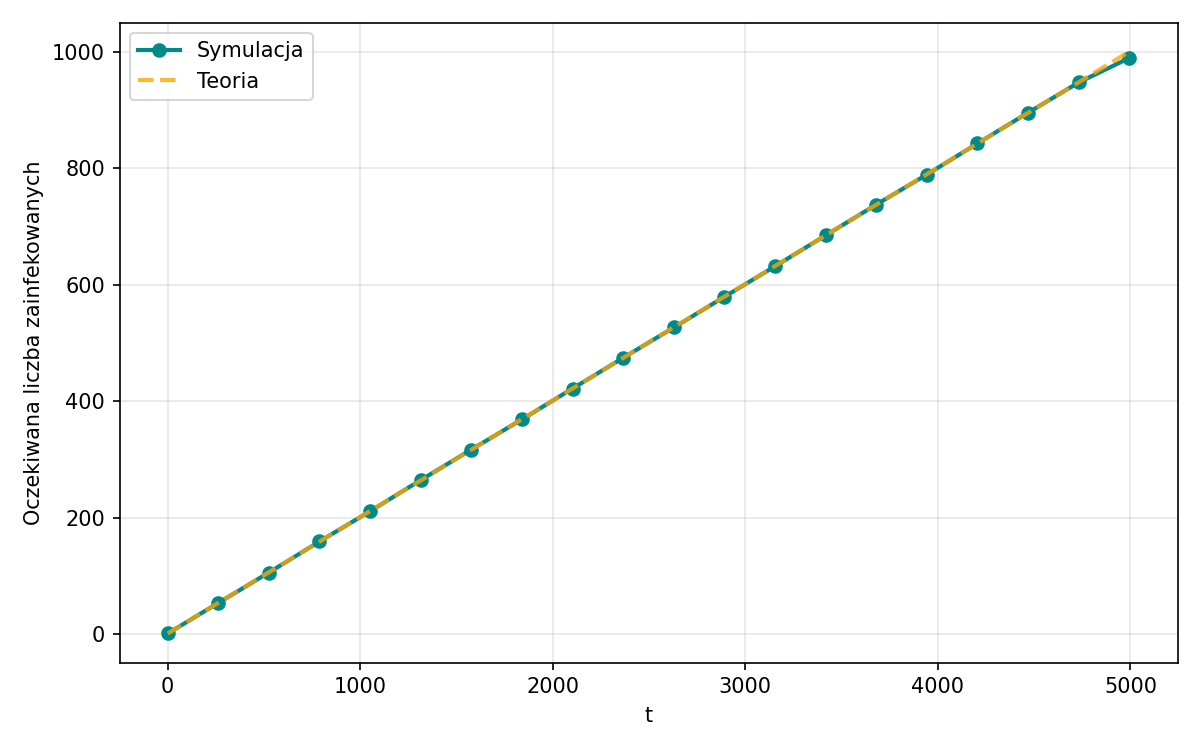
\includegraphics[width=1\textwidth]{../img/path/final_infection_expectations.png}
    \caption{$\mathbb{E}[Y_t]$ dla $\mathrm{P_n}$ w funkcji $t$}
\end{figure}
\begin{figure}[h!]
    \centering
    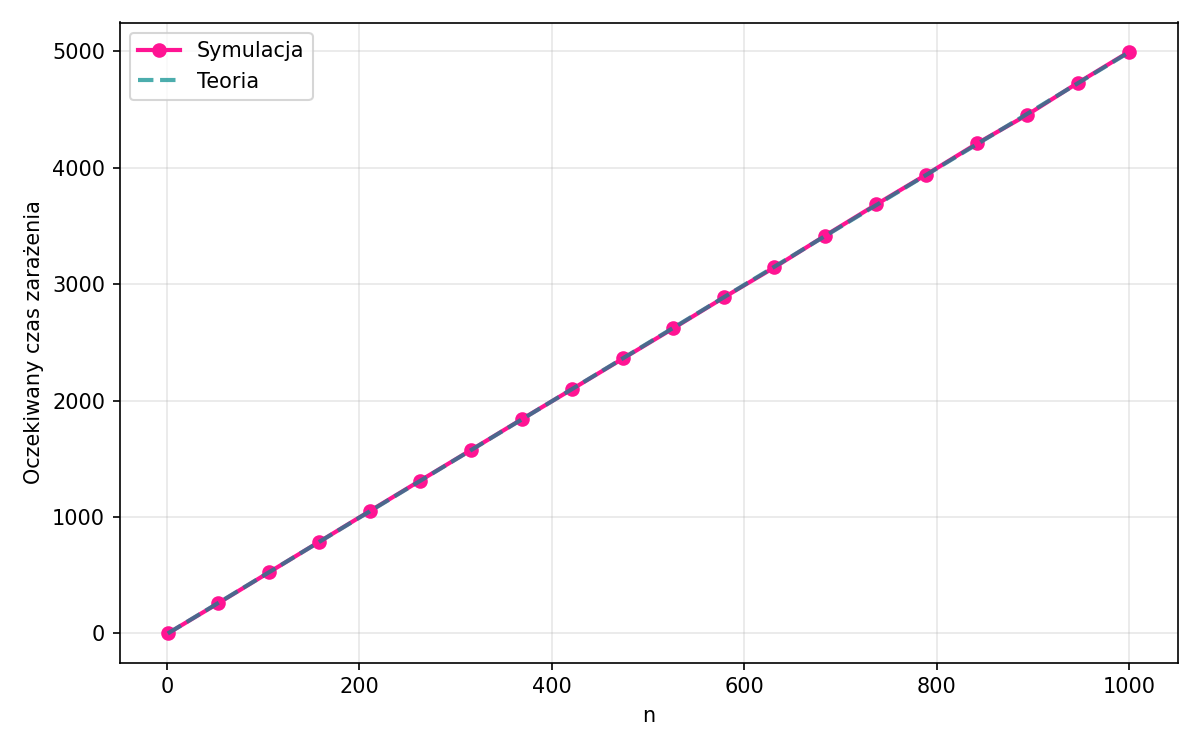
\includegraphics[width=1\textwidth]{../img/path/full_infection_expectation.png}
    \caption{$\mathbb{E}[Z]$ dla $\mathrm{P_n}$ w funkcji $n$}
\end{figure}
Wyniki eksperymentu niemal idealnie pokrywają się z przewidywanymi kształtami, to jest $1+tp$ dla $\mathbb{E}[Y_t]$ oraz $\frac{n-1}{p}$ dla $\mathbb{E}[Z]$.


\section{Analiza dla grafów gwiazd}

Następnie rozpatrzmy rodzinę grafów gwiazd $\mathrm{S}_n$. Niech źródłem będzie centralny wierzchołek grafu, to jest $s=0$. Propagacja rozchodzi się tutaj po każdym ramieniu gwiazdy niezależnie. Stąd mamy $X_v \sim \mathrm{Geo}(p)$ dla każdego $v\in\{1,2,\dots,n\}$. Ponadto zmienne $X_1,X_2,\dots,X_n$ są od siebie niezależne. Mamy więc
\[
    \mathbb{E}[X_v]=\frac{1}{p}, \quad \mathrm{Var}[X_v]=\frac{1-p}{p^2}
\]

Kwestia $Y_t$ jest również dość prosta. Skoro propagacja działa na każdym wierzchołku niezależnie to zmienna $Y_t$ jest wynikiem $n$ prób Bernoulliego. Sukces pojedynczej próby to prawdopodobieństwo, że zmienna $X_v$ o rozkładzie geometrycznym po conajwyżej $t$ jednostkach czasu osiągnie swój sukces. A więc jest to $\mathbb{P}[X_v\le t]=1-q^t$. Podsumowując mamy
\[
    Y_t = 1 + B_t, \quad B_t \sim \mathrm{Bin}(n, 1-q^t)
\]
Stąd oczywiście otrzymujemy 
\[
    \mathbb{E}[Y_t] = 1 + n\cdot (1-q^t)
\]
Przejdźmy teraz do zmiennej $Z$. Przypomnijmy, że $Z=\max\{X_1,X_2,\dots,X_n\}$. Skoro zmienne te są IID, to z \Cref{F:max_CDF} mamy 
\[
    \mathbb{P}[Z\le t] = (1-q^t)^n
\]
Policzmy teraz wartość oczekiwaną całkowitego zainfekowania grafu. 
\begin{align*}
\mathbb{E}[Z] 
&= \sum_{k=1}^{\infty} \mathbb{P}[Z\ge k] 
 = \sum_{k=1}^{\infty} 1 - \mathbb{P}[Z\le k-1]
 = \sum_{k=1}^{\infty}  1 - (1-q^{k-1})^n  \\
&= \sum_{k=0}^{\infty}  1 - (1-q^k)^n 
 = \sum_{k=0}^{\infty} \left( 1 - \sum_{j=0}^{n} \binom{n}{j} (-1)^j q^{kj} \right) \\
&= \sum_{k=0}^{\infty} \sum_{j=1}^{n} \binom{n}{j} (-1)^{j+1} q^{kj} = \sum_{j=1}^{n} \sum_{k=0}^{\infty} \binom{n}{j} (-1)^{j+1} (q^j)^k \\
&= \sum_{j=1}^{n} \binom{n}{j} \frac{(-1)^{j+1}}{1-q^j}
\end{align*}
Nie jest to jednak przyzwoity wynik i nie ma postaci zwartej. Spróbujmy zatem wyznaczyć asymptotykę $\mathbb{E}[Z]$. Mamy $\mathbb{E}[Z] = \sum_{k=0}^{\infty}  1 - (1-q^k)^n$. \cref{F:approximation_of_sum_by_an_integral} umożliwia oszacowanie tej sumy. Połóżmy $f(x) = 1 - (1 - e^{-\alpha x})^n$ gdzie $\alpha = -\log(q)$. Oczywiście $f(0)=1$ , $f(\infty)=0$ oraz $f$ jest malejąca a więc
\[
    \int_{0}^{\infty} f(x) \; \mathrm{d}x \le \mathbb{E}[Z] \le  1 + \int_{0}^{\infty} f(x) \; \mathrm{d}x
\]
Podstawiamy $u = 1 - e^{-\alpha x}$. Wtedy $\mathrm{d}u = \alpha e^{-\alpha x} \; \mathrm{d}x$, 
a więc $\mathrm{d}x = \frac{1}{\alpha}\cdot\frac{1}{1-u} \; \mathrm{d}u$. 
Ponadto $u(0) = 0$, $u(\infty) = 1$ (bo $\alpha > 0$). 
Zatem całka ma postać:
\[
 \frac{1}{\alpha} \int_{0}^{1} \frac{1 - u^n}{1 - u} \; \mathrm{d}u
= \frac{1}{\alpha} \int_{0}^{1} \sum_{j=0}^{n-1} u^j \; \mathrm{d}u
= \frac{1}{\alpha} \sum_{j=0}^{n-1} \frac{1}{j+1}
= \frac{H_n}{\alpha}
\]
Zauważmy, że $-\log(q)=\log(\frac{1}{1-p})$ a więc ostatecznie dostajemy:
\[
    \frac{H_n}{\log(\frac{1}{1-p})} \le \mathbb{E}[Z] \le \frac{H_n}{\log(\frac{1}{1-p})} + 1
\]
Stąd mamy asymptotyczny przewidywany czas zarażenia grafu $\mathrm{S}_n$:
\[
    \mathbb{E}[Z] \sim \frac{H_n}{\log(\frac{1}{1-p})}
\]
Przeprowadźmy teraz symulacje. Ustalmy $p=0.2$, $n=1000$. Dla każdego $t\in\{1, 2, \dots, \log(n)\}$ wykonajmy $2000$ powtórzeń propagacji na $\mathrm{S}_n$. Potem dla $n\in\{1,2,\dots,1000\}$ tak samo dla $\mathbb{E}[Z]$. 
\begin{figure}[h!]
    \centering
    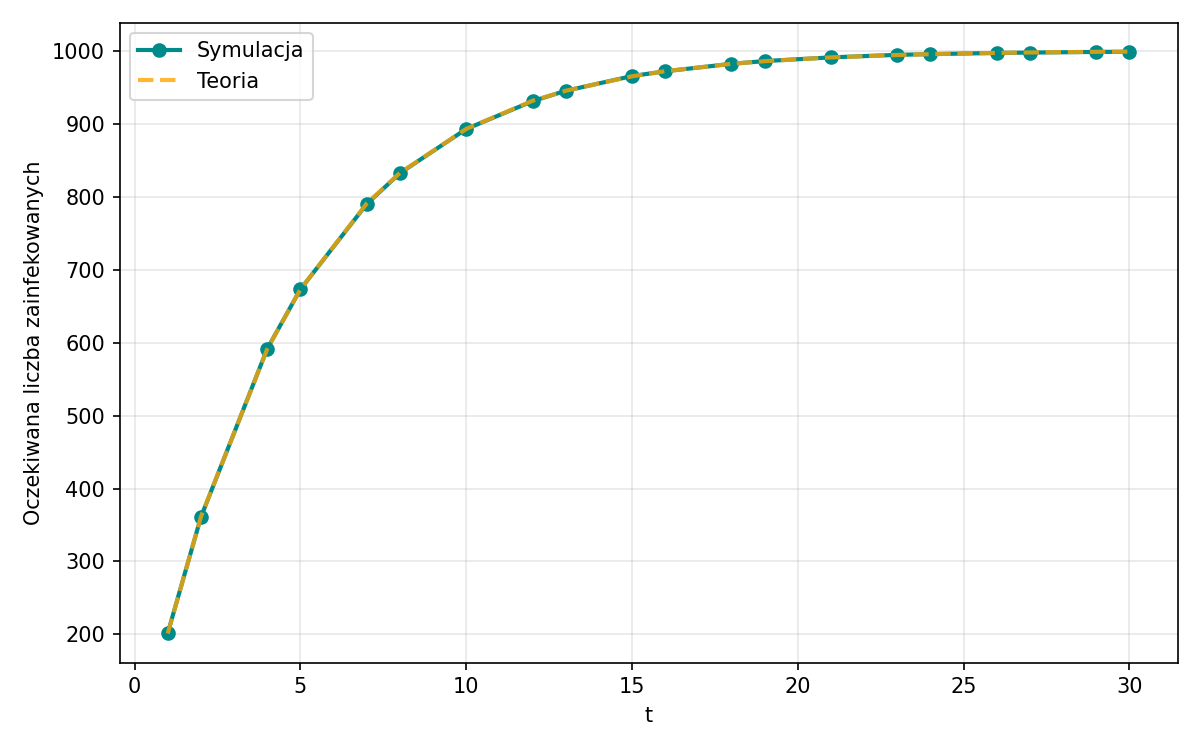
\includegraphics[width=1\textwidth]{../img/star/final_infection_expectations.png}
    \caption{$\mathbb{E}[Y_t]$ dla $\mathrm{S_n}$ w funkcji $t$}
\end{figure}
\begin{figure}[h!]
    \centering
    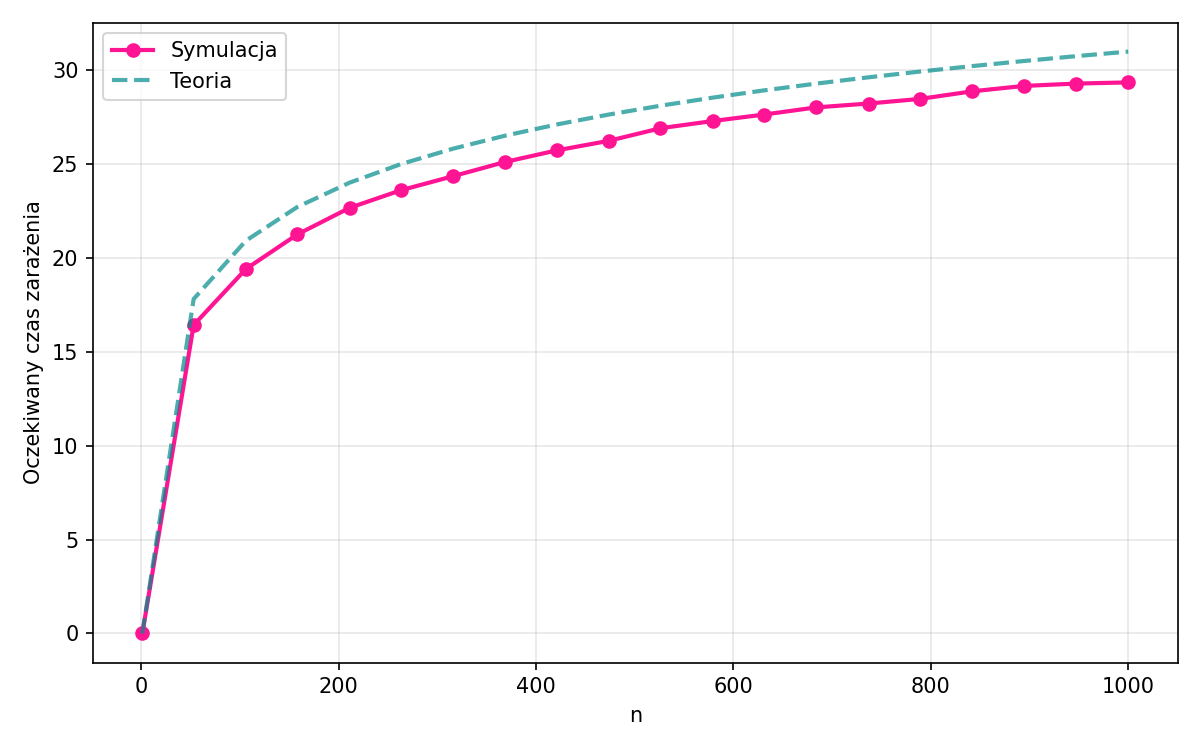
\includegraphics[width=1\textwidth]{../img/star/full_infection_expectation.png}
    \caption{$\mathbb{E}[Z]$ dla $\mathrm{S_n}$ w funkcji $n$}
\end{figure}
Dla $\mathbb{E}[Y_t]$ po raz kolejny mamy idealne dopasowanie. Dla $\mathbb{E}[Z]$ zaś numeryczna wartość jest o około $1$ mniejsza niż przewidywana, co jest dobrym wynikiem.


\section{Ograniczenia na czasu zarażenia}
Po rozważeniu dwóch rodzin grafów dostrzegamy znaczną różnicę w wartościach oczekiwnaych zmiennych $Y_t$ oraz $Z$. Dla grafów ścieżkowych minimalna liczb rund potrzebnych do zainfekowania całego grafu wynosi $t=n-1$ natomiast dla gwiazd jest to zaledwie $t=1$. Widzimy, że w pewnym sensie najlepszy przypadek sprzyjający szybkiej propagacji jest taki, w którym źródło $s$ jest połączone z wszyskimi pozostałymi wierzchołkami grafu. Z drugiej strony najgorsza sytuacja ma miejsce, jeśli istnieje daleko oddalony węzeł, szczególnie z mało liczbą ścieżek do niego prowadzących, tak jak dla grafów ścieżkowych. Teraz postaramy się uogólnić tą obserwację. 

\begin{theorem}\label{T:montonicity_of_total_infection}
Niech $G=(V,E)$ będzie grafem spójnym a $G'=(V,E')$ spójnym podgrafem $G$. Załóżmy, że $\mathbf{X}$ jest procesem stochastycznym w modelu SI na $G$ oraz $G'$ jednocześnie z tym samym źródłem $s\in V$. Jeśli przez $Z$ oznaczymy czas całkowitego zarażenia $G$ i odpowiednio przez $Z'$ dla $G'$ to wtedy zachodzi nierówność $\mathbb{E}[Z]\le\mathbb{E}[Z']$. 
\end{theorem}

Intuicyjnie sprawa jest oczywista. Mając mniej krawędzi w grafie potrzebujemy więcej czasu na rozprzestrzenienie się w nim informacji.

\begin{proof}
Oznaczmy przez $\mathcal{I}_t$ zainfekowane wierzchołki w $G$ a przez $\mathcal{I}_t'$ w $G'$. Wtedy $\mathcal{I}'_t\subseteq\mathcal{I}_t$ dla dowolnego $t\in\mathbb{N}$. Ponadto mamy
\[
    Z = \min\{t\in\mathbb{N} : \mathcal{I}_t=V\},  \quad Z' = \min\{t\in\mathbb{N} : \mathcal{I}_t'=V\}
\]
Niech $Z' = \tau$. Wtedy $\mathcal{I}'_\tau =V$ a więc $V\subseteq \mathcal{I}_t$. Zatem $\mathcal{I}_\tau = V$ i $Z\le \tau$. Korzystając z \Cref{F:montonicity_of_expectation} dostajemy $\mathbb{E}[Z]\le\mathbb{E}[Z']$.
\end{proof}

W praktyce oznacza to, że jeżeli znamy średni czas zainfekowania dowolnego podgrafu $G$ to znamy ogarniczenie górne na czas dla całego grafu. Postarajmy się teraz oszacować sensownie z góry  wartość $\mathbb{E}[Z]$ dla dowolnego grafu.

\begin{theorem}\label{T:upper_bound_on_EZ}
Niech $G=(V,E)$ będzie grafem o $n$ wierzchołkach zaś $s\in V$ będzie ustalonym źródłem. Ozanczmy przez $\ell = \epsilon(s)$. Wtedy zachodzi
\[
    \mathbb{E}[Z] \le \ell  + \ell \cdot \frac{\log(\frac{n-1}{\ell}) + 1}{\log(\frac{1}{1-p})}
\]
\end{theorem}

\begin{proof}
Dla $0\le j \le \ell$ kładziemy $A_j = \{v \in V : \mathrm{d}(s,v) = j\}$ oraz $n_j= |A_j|$. Oczywiście $n_0=1$ a więc $n_1+\cdots+ n_\ell = n -1 $. Dalej zdefiniujmy zmienne losowe $T_j = \min\{t\in\mathbb{N} : A_j \subseteq \mathcal{I}_t\}$. Zmienna $T_j$ określa czas potrzebny do zainfekowania wierzchołków oddalonych o $j$ od źródła. Udowodnijmy teraz przydatny lemmat.

\begin{lemma}\label{L:helper_lemma}
Niech $U_j = T_j - T_{j-1}$ dla $1 \le j \le \ell$. Wtedy:
\[
    \mathbb{E}[U_j] \le \frac{H_{n_j}}{\log(\frac{1}{1-p})} + 1
\]
\end{lemma}
\begin{proof}
$U_j$ to czas potrzebny na zarażenie wierzchołków $A_j$ podczas gdy $A_{j-1}$ są już zarażone. Wybierzmy podgraf $G'$ w taki sposób, żeby każdy wierzchołek z $A_j$ był połączony dokładnie jedną krawędzią z którymś z wierzchołków ze zbioru $A_{j-1}$. Wtedy rozkład propagacji na $G'$ jest izomorficzny z tym dla $\mathrm{S}_{n_j}$ bo $n_j=|A_j|$. Pamiętajamy, że $\frac{H_{n_j}}{\log(\frac{1}{1-p})} + 1$ jest ograniczeniem górnym na całkowity czas zarażenia grafu gwiazdy oraz wykorzystując \cref{T:montonicity_of_total_infection} dostajemy porządany wynik.
\end{proof}

Wrócmy do udowadniania ograniczenia na $\mathbb{E}[Z]$. Mamy $T_\ell = \sum_{j=1}^{\ell} U_j$ a więc:
\begin{equation*}
\begin{aligned}
\mathbb{E}[Z] 
&\le \mathbb{E}[T_\ell] 
  = \mathbb{E}\left[\sum_{j=1}^{\ell} U_j\right] 
  = \sum_{j=1}^{\ell} \mathbb{E}[U_j] 
  \le \sum_{j=1}^{\ell} \frac{H_{n_j}}{\log(\frac{1}{1-p})} + 1 \\
&= \ell + \frac{1}{\log(\frac{1}{1-p})} \sum_{j=1}^{\ell} H_{n_j} 
  \le \ell + \frac{1}{\log(\frac{1}{1-p})} \sum_{j=1}^{\ell} 1 + \log(n_j) \\
&= \ell + \frac{\ell}{\log(\frac{1}{1-p})} \cdot \left(1 + \sum_{j=1}^{\ell} \log(n_j) \right) \\
&= \ell + \frac{\ell}{\log(\frac{1}{1-p})} \cdot \left(1 + \log \left(\prod_{j=1}^{\ell} n_j\right)\right) \\
&\le \ell + \frac{\ell}{\log(\frac{1}{1-p})} \cdot \left(1 + \log \left(\frac{1}{\ell} \sum_{j=1}^{\ell} n_j\right) \right) \\
&= \ell + \frac{\ell}{\log(\frac{1}{1-p})} \cdot \left(1 + \log \left(\frac{n-1}{\ell}\right) \right) = \ell  + \ell \cdot \frac{\log(\frac{n-1}{\ell}) + 1}{\log(\frac{1}{1-p})}.
\end{aligned}
\end{equation*}
gdzie w linijce pierwszej wykorzystujemy monotoniczności propagacji, w drugiej \cref{F:harmonic_upper_bound} a w piątej z nierówności między średnimi (\ref{F:AM_GM}).
\end{proof}

Porównajmy przed chwilą udowodnione twierdzenie z poprzednimi wynikami. Dla rodziny $\mathrm{P}_n$ mamy $\ell = n - 1$. Dodatkowo korzystając z \Cref{F:log_vs_x} mamy
\[
    \mathbb{E}[Z] \le (n-1) \cdot \left(1 + \frac{1}{p} \right)
\]
Przypomnijmy, że faktyczna wartość oczekiwana jest równa $\frac{n-1}{p}$ więc oszacowanie jest dość ostre. Z kolei dla rodziny $\mathrm{S}_n$ mamy $\ell=1$ oraz $n+1$ wierzchołków a więc
\[
    \mathbb{E}[Z] \le 1 + \frac{\log(n) + 1}{\log(\frac{1}{1-p})}
\]
Ponownie oszacowanie jest dość dokładne. Wynik ten zdaje się być dobry dla grafów rzadkich.


\section{Analiza dla drzew}

Rozważmy drzewo $G = (V, E)$ oraz ustalony wierzchołek początkowy $s \in V$, 
który traktujemy jako korzeń drzewa. Dla $v\in V$ oznaczmy  $d_v=\mathrm{d}(s,v)$. Ustalmy $v\in V$. Skoro $G$ jest drzewem to istnieje dokładnie jedna ścieżka od $s$ do $v$, powiedzmy $s,v_1,\dots,v_k, v$. Ponieważ infekcja rozprzestrzenia się od korzenia $s$ wzdłuż krawędzi drzewa, 
każde zakażenie wymaga sukcesu w niezależnym doświadczeniu Bernoulliego o prawdopodobieństwie $p$.
W konsekwencji, aby infekcja dotarła z $s$ do $v$, 
musi wystąpić $\mathrm{d}_v$ kolejnych sukcesów. Zatem rozkład $X_v$ pokrywa się z rozkładem tej zmiennej dla grafu $\mathrm{P}_{d_v+1}$ na wierzchołkach $\{s,v_1,\dots,v_k, v\}$. Stąd 
\[
    X_v\sim \mathrm{NegBin}(\mathrm{d}_v,p)
\]
oraz
\[
    \mathbb{E}[X_v] = \frac{\mathrm{d}_v}{p}, \quad \mathrm{Var}[X_v] = \frac{\mathrm{d}_v\cdot(1 - p)}{p^2}
\]
\begin{lemma}\label{L:Formula_EYt}
Dla dowolnego $t\in\mathbb{N}$ wartość oczekiwana zmiennej $Y_t$ wyraża się wzorem
\[
    \mathbb{E}[Y_t] = \sum_{v\in V} \mathbb{P}[X_v \le t]
\]    
\end{lemma}

\begin{proof}
Mamy $Y_t=|\{v\in V: X_v \le t\}|$ zatem $Y_T=\sum_{v\in V}  \mathbf{1}_{\{X_v\le t\}}$. Nakładając na tą równość operator $\mathbb{E}$ otrzymujemy:
\[
    \mathbb{E}[Y_t] = \mathbb{E}\left[ \sum_{v\in V}  \mathbf{1}_{\{X_v\le t\}}\right]= \sum_{v\in V} \mathbb{E}[\mathbf{1}_{\{X_v\le t\}}] = \sum_{v\in V} \mathbb{P}[X_v \le t]
\]    
\end{proof}

Przejdźmy teraz to obliczania średniej liczby zainfekowanych wierzchołków w czasie $t$. Oznaczmy przez $F(t;m,p)$ dystrybuante zmiennej o rozkładzie $\mathrm{NegBin}(m,p)$. Z \Cref{L:Formula_EYt} otrzymujemy
\[
    \mathbb{E}[Y_t] = \sum_{v\in V} F(t; d_v, p)
\]
Połóżmy $n_j = |\{v\in V: d_v=j\}|$ dla $0\le j \le h$. Wtedy 
\[
    \mathbb{E}[Y_t] = \sum_{j=0}^{h} n_j\cdot F(t; j, p)
\]
Ponadto gdy $t<j\le h$ to $F(t; j, p)$, bo żaden wierzchołek w odległości od korzenia większej niż liczba rund nie może zostać zarażony. Możemy więc zmniejszyć granice sumowania 
\[
    \mathbb{E}[Y_t] = \sum_{j=0}^{\min\{h,t\}} n_j\cdot F(t; j, p)
\]
Oszacujmy teraz średni czas całkowity czas propagacji drzewa.
Niech $\{u_1,\dots, u_m\}$ będą liściami w $G$. Wtedy mamy $Z = \max_{1\le i \le m} X_{u _i}$.
Zauważmy, że $\epsilon(s) = \max_{1\le i \le m} \mathrm{d}_{u_i}$ i jest to wysokość drzewa. Oznaczmy ją przez $h$. Z nierówności Jensena (\cref{F:Jensen}) dla funkcji $\max\{x_1,\dots,x_m\}$ otrzymujemy
\[
    \mathbb{E}[Z]=\mathbb{E}[\max_{1\le i \le m} X_{u _i}] \ge \max_{1\le i \le m} \mathbb{E}[X_{u _i}] = \max_{1\le i \le m} \frac{\mathrm{d}_{u_i}}{p} = \frac{h}{p}
\]
Największą wysokość ma drzewo, które jest ścieżka i wtedy $h=n-1$. Zgodnie z poprzednimi wyliczeniami jest to dobre oszacowanie. Aby ogarniczyć $\mathbb{E}[Z]$ z góry skorzystamy z \Cref{T:upper_bound_on_EZ}:
\[
    \mathbb{E}[Z] \le h  + h \cdot \frac{\log(\frac{n-1}{h}) + 1}{\log(\frac{1}{1-p})}
\]


\section{Analiza dla grafów pełnych}

Graf pełny $\mathrm{K}_n$ intuicyjnie powinien mieć najszybszą propagację ze względu na maksymalną liczbę krawędzi. Początkowo rozkład $X_v$ pokrywa się z rozkładem gwiazdy natomiast w każdej kolejnej rundzie mocno się komplikuje. Jeśli bowiem $Y_t=a$ to $\mathbb{P}[X_v = t+1] = 1 - q^a$. Ta olbrzymia liczba powiązań uniemożliwia jakiekolwiek sensowne wyznaczenie rozkładu $X_v$. Podejdźmy do problemu narazie heurystycznie. Zauważmy, że jeśli $Y_1=a$ to rozkład zmiennej $Y_2$ wynosi $Y_2 = a + B$ dla $B \sim \mathrm{Bin}(n-a, 1-q^n)$. Zatem 
\[
    \mathbb{E}[Y_2\mid Y_1 = a] = n\cdot (1-q^a) + aq^a
\]
Skoro rozkład $Y_1$ pokrywa się z tym dla $\mathrm{S}_{n-1}$ to
\[
    \mathbb{E}[Y_1]\approx\frac{H_{n-1}}{\log(\frac{1}{1-p})} \approx \frac{\log(n)}{\log(\frac{1}{q})} = \log_{q}\left(\frac{1}{n}\right)
\]
Powinniśmy się spodziewać, że również $a \approx \mathbb{E}[Y_1]$ a co za tym idzie $q^a \approx \frac{1}{n}$ jak również
\[
    \mathbb{E}[Y_2\mid Y_1 = a] \approx n \cdot (1 - \frac{1}{n}) + \frac{1}{n} \cdot\log_{q}\left(\frac{1}{n}\right) \approx n - 1
\]
Spodziewamy się zatem, że zaledwie po dwóch rundach cały graf $\mathrm{K}_n$ będzie zainfekowany. Zweryfikujmy teraz ten heurystyczny argument symulacją w Pythonie. Ustalmy $p=0.2$ i dla $n\in\{2,3,\dots,1000\}$ odpalmy propagację. 
\begin{figure}[h!]
    \centering
    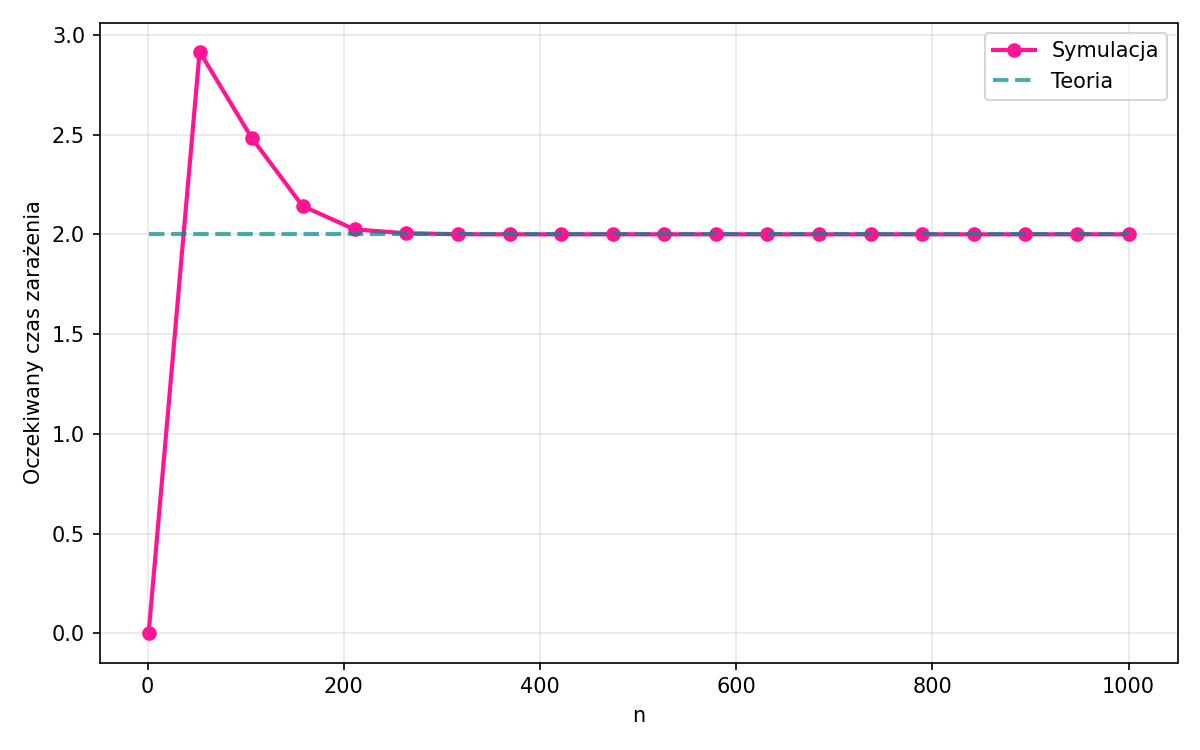
\includegraphics[width=1\textwidth]{../img/complete/full_infection_expectation.png}
    \caption{$\mathbb{E}[Z]$ dla $\mathrm{K_n}$ w funkcji $n$}
\end{figure}
Widzimy, że dla $n>200$ mamy $\mathbb{E}[Z] \approx 2$. Możemy więc wysunąć hipotezę: Dla grafu $\mathrm{K}_n$ mamy:
\[
    \lim_{n\to\infty} \mathbb{E}[Z] = 2
\]